\chapter{History}\label{history}

This chapter discusses the space shuttle program in order to provide an overview of the information the security markets might have incorporated into prices of the shuttle firms. The chapter begins with an overview of the shuttle program and how the current design came about. It is followed by a section on mission 51-L, the {\em Challenger} mission that was lost. Following this is a very detailed discussion of the accident itself to illustrate what was eventually determined to have happened. The purpose of this section is to show that the true events could not have been discerned on the day of the accident. In fact, the accident appeared to be caused by many things other than what really caused it. The sources of incorrect information about the cause of the accident are covered. Finally, the chapter closes with a discussion of what investigators determined to be the actual cause of the accident and how widespread knowledge of this possible failure path was known.

\section{Space Shuttle}

The space shuttle program was initiated in the 1960s to provide relatively inexpensive access to space. The giant Apollo program was winding up, and the war in Viet Nam required an increasing portion of the budget. NASA needed to find a cheaper means of transportation to space when they devised the Space Transport System or STS. The lower costs came about from complete reusability of the components, contrasted with the Apollo program that required giant disposable rockets. Complete reusability would make space travel more economical, and, it was hoped, would allow the program to pay for itself.\footnote{NASA envisioned selling cargo space on the STS for satellites, military and commercial.} A problem remained, however; the program needed Congressional approval. If the system were entirely reusable, it would entail development costs (1970) of \$10 to \$12 billion (spread over seven or eight years) \cite[p. 57]{lewis}. Congress and the Office of Management and Budget refused to go along with this plan, forcing NASA to redesign the system.

In order to receive Congress's approval, NASA shifted the costs from development to operation. The craft would be cheaper to develop, but would cost a lot more to operate. In doing so, NASA scrapped the idea of a manned first stage that would carry the orbiter (riding piggy back) to orbit and then return to earth. The manned first stage was replaced by a combination of solid rocket boosters and a liquid tank that would contain fuel for the orbiter's main engines (located at the aft area of the orbiter and fed by a series of pipes from the external tank). They also scrapped the idea of jet engines in the orbiter,\footnote{Air-burning jet engines would allow the orbiter more flexibility in returning to earth or aborting a mission but would add a lot of weight and design effort.} complete reusability, and an orbiter with a large wingspan.

These changes put the final development costs at \$6.2 billion in 1972 dollars \cite[vol. 1, p. 4]{rogers}. The final system, the one in use today, consists of a delta-winged orbiter mounted on a large, rust-colored tank. Mounted to the tank are two solid rocket boosters, the largest ever made. The external tank that the orbiter is attached to contains three smaller tanks. The first, located at the top of the tank, contains liquid oxygen, some 143,000 gallons at -297 degrees Fahrenheit. The other tank, located in the aft, or tail, section of the external tank contains liquid hydrogen at -423 degrees Fahrenheit \cite[vol. 1, p. 8]{rogers}. The third, called the intertank, sits between the liquid oxygen and hydrogen tanks and houses instrumentation needed to assure operation of the external tank. These three tanks comprise the external tank, which is manufactured by Martin Marietta and is 154 feet long and 27$\frac{1}{2}$ feet in diameter \cite[vol. 1, p. 8]{rogers}.

The main shuttle engines feed from this external tank through a maze of pipes, pumps, and valves. The engines fire for about 8$\frac{1}{2}$ minutes after liftoff and can generate 375,000 pounds of thrust (at sea level) at 100 percent throttle, burning a mixture of liquid hydrogen and liquid oxygen supplied from the external tank \cite[vol. 1, p. 7]{rogers}. The main engine's range of operations extends from 65 percent to 104 percent of throttle \cite[vol. 1, p. 8]{rogers}. The engines themselves are manufactured by Rocketdyne, a subsidiary of Rockwell International, the manufacturer of the orbiter.

Attached to the external tank are two of the largest solid rocket boosters ever manufactured. They provide about 80 percent of the total thrust and burn for roughly two minutes until exhausted. The boosters themselves are made up of four segments that are shipped to NASA by rail. The segmented design allows for easier shipment to and from the Morton Thiokol's (the manufacturer's) plant in Utah to NASA. The SRBs, as the Solid Rocket Boosters are called, are 116 feet long when the four segments are joined and held together with 177 steel pins. The joint (called a field joint) itself is made up of a tang and clevis; a clevis is a U-shaped part into which a tang fits. The joint is depicted in Figure~\ref{fieldj}.

\begin{figure}[p]
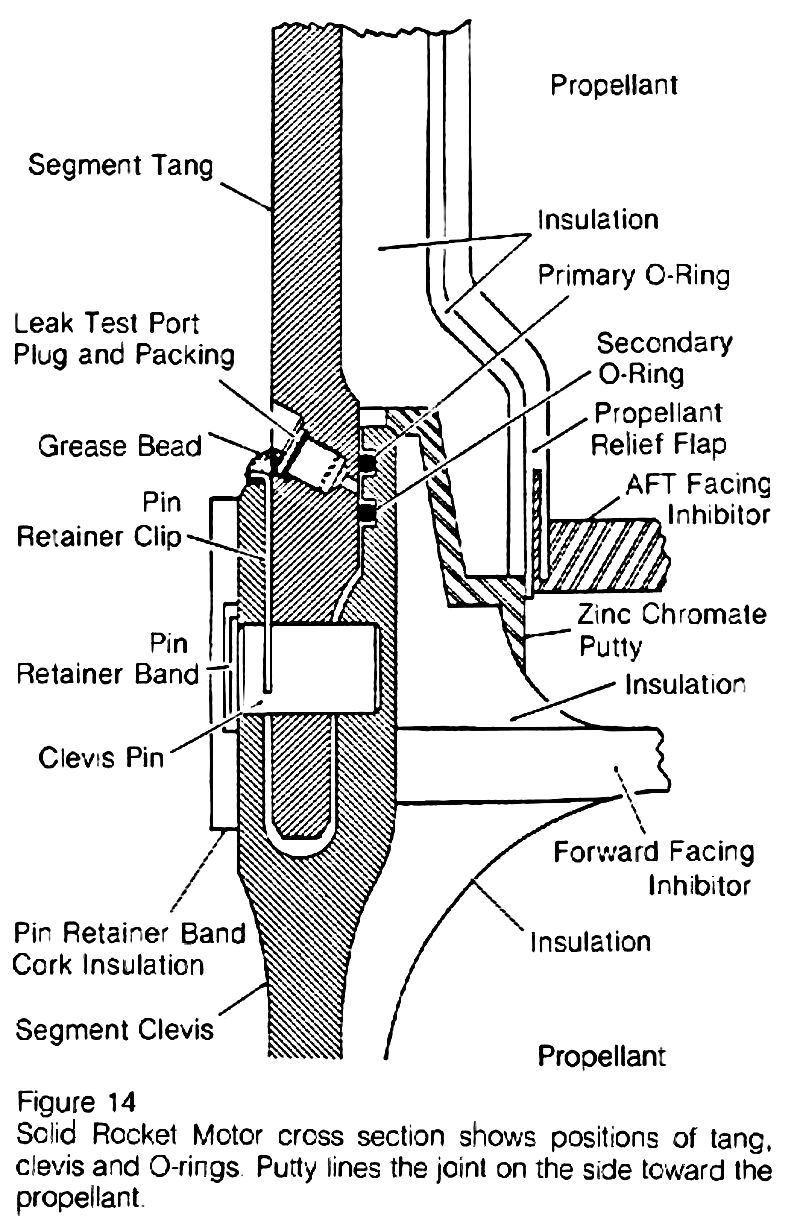
\includegraphics{RogersCommission-v1p57.jpg}
 %\vspace{4.75in}
\caption{The solid rocket booster field joint
\protect\cite[vol. 1, p. 57]{rogers}.}
\label{fieldj}
\end{figure}

The gap between the tang and clevis is sealed with a pair of rubber rings called O-rings. The segmented design represents the weakness in the solid rocket boosters. By joining the boosters together in four segments, four escape paths for the hot gasses are provided. The O-rings are supposed to provide a sealing action to prevent these hot gasses from escaping through a field joint, but the O-rings were never meant to survive the heat of the gasses themselves. Zinc chromate putty is packed between the solid rocket core and the O-rings. The putty is flame-proof, and, in theory, should become plastic and melt around the O-rings, protecting them from the heat.


This current design represents a compromise over the original design. Higher operating costs (not complete reusability like the original design) were traded off for much lower development costs (half of the original amount). The compromise represented a compromise in crew safety as well. Although the SRBs provided more thrust than an equally sized liquid propellant system, they exposed the crew to a two minute window when escape was ``nonsurvivable'' \cite[p. 59]{lewis}. Yet solid rocket technology was considered one of the most reliable around. In fact, ``before the Challenger accident, it was believed by some shuttle observers\ldots that the SRBs were as safe and reliable as rockets could be'' \cite[pp. 63--64]{lewis}. Also, ``the perception that the SRBs were virtually foolproof was widely shared in NASA during shuttle development and was strongly communicated to the news media correspondents'' \cite[p. 64]{lewis}.

\section{Mission 51-L}

Flight 51-L was the {\em Challenger} mission that was lost. NASA's numbering system designated this mission 51-L with the first digit (``5'') representing the fiscal year that the launch was originally supposed to occur. The second digit indicated where the launch was to occur (here ``1'' represents Kennedy Center). The third, a letter, specifies which launch in that fiscal year (with ``A'' as the first mission). Mission 51-L was unique because Christa McAuliffe, the first ``Teacher In Space,'' was aboard. She and her six other crewmates\footnote{They were Commander Francis R. (Dick) Scobee, Pilot Michael John Smith, Mission Specialist One Ellison S. Onizuka, Mission Specialist Two Judith Arlene Resnik, Mission Specialist Three Ronald Erwin McNair, and Payload Specialist Two Gregory Bruce Jarvis. Christa McAuliffe's title was Payload Specialist One.} faced four postponements and one scrub of the mission. The flight was originally scheduled for July of 1985 \cite[vol. 1, p. 10]{rogers}, but changes in payloads pushed the date back to November, 1985. More delays occurred, and the mission was moved to January of 1986. As the mission was pushed back again and again, there was increasing pressure to launch to keep up with NASA's ambitious launch schedule. NASA also faced a constraint in that a payload needed to be launched by March to investigate Halley's Comet; a {\em Challenger} launch delay could prevent this comet probe from being launched in March.

The launch was finally scheduled for Tuesday, January 28, 1986. The temperature at the time of launch was 36 degrees Fahrenheit, causing some concern among the shuttle's contractors. Executives of Rockwell International, the builder of the orbiter, expressed concern about the ice on the launch pad.\footnote{The launch structure was covered with ice because, fearing frozen pipes, NASA officials decided to allow water to trickle from the water pipes.} The concern centered around the possibility that ice might break off under the enormous acoustic shocks when the engines are ignited. Falling ice could dislodge the heat resistant tiles that line the underside of the shuttle. The tiles protect the orbiter from the heat of re-entry.

NASA had sent an ``ice team'' to investigate the problem. The ice team measured the temperature of the right solid rocket booster and found it to be about 19 degrees Fahrenheit, well below the manufacturer's (Morton Thiokol's) contracted low temperature of 40 degrees Fahrenheit. The contract between NASA and Thiokol stipulated that the SRBs operate above 40 degrees Fahrenheit. The temperature finding was not reported up the chain of command.

Morton Thiokol's engineers\footnote{Morton Thiokol manufactures the solid rocket boosters.} were concerned as well about the low temperature. The engineers had never fired test rockets at such a low temperature and were concerned about something they observed in January, 1985. The January, 1985 launch was unique because it had been the coldest to date. Although they had no statistical data to suggest there was a correlation, the engineers felt there was a correspondence between temperature and the O-rings not sealing. By not sealing, the O-rings had allowed hot gasses to escape through the joint, burning (eroding) several hundredths of an inch from the secondary O-ring. Damage occurred in both solid rocket boosters in the January, 1985 launch.

The engineers were overridden, however, and Thiokol gave approval for the launch. The engineers were put in the position of having to prove that the O-rings would fail, rather than prove that they would work. There was also no launch constraint for temperature; no one really knew how cold it could be.

\section{The Accident}

The Space Shuttle {\em Challenger}, Mission 51-L of Tuesday, January 28, 1986, had been postponed four times and scrubbed once. When the craft was finally launched at 11:38 am EST, the mission progressed normally until T+73 seconds\footnote{This notation (T+73 seconds) refers to 73 seconds after launch.} when the {\em Challenger} exploded and killed all seven crew members. It was not immediately obvious what had happened, and some of the people on the ground thought the smoke indicated the planned-for separation of the orbiter from the external tank.

In spite of the uncertainty about the cause of the problem, there was visual indication of some problems immediately after ignition of the solid rocket boosters; no one noticed the problem until enhanced photographs of the shuttle were analyzed. The right SRB emitted several puffs of black smoke at 0.678 seconds into the launch (T+0.678). A total of nine puffs of smoke appeared between 0.836 and 2.500 seconds at a lower joint on the right SRB \cite[vol. 1, p. 19]{rogers}. The smoke's color suggested that the O-rings between joins had burned, causing what is called ``blow by.'' It appears that no one at NASA noticed this blow by, and had anyone, it would have been impossible to stop the solid rockets, as they burn continuously until they are exhausted. At 2.733 seconds, the last positive evidence of smoke was visible from the right aft field joint;\footnote{The smoke first appeared on camera E60, a 16mm motion picture camera with a 32mm lens. The camera was located 1270 feet from the shuttle and shot 100 frames per second \cite[vol. 3, p. N-9]{rogers}.} the shuttle was moving upward and the aft smoke intermingled with plumes from the rocket.

All this time the shuttle's main engines had been burning (they were ignited 6.6 seconds before launch in order to get up to full thrust by the time of launch). The shuttle system was bolted to the launch structure, which bends under the force of the main engines. The launch structure bends back in what is called a ``twang'' motion. At this time the pyrotechnic bolts are exploded, releasing the launch structure's stored energy. The Rogers Commission report explains, ``the maximum structural loads on the aft field joints [where the black smoke appeared] of the Solid Rocket Boosters occur during the `twang,' {\em exceeding even those of the maximum dynamic pressure period experienced later in flight} [emphasis added]'' \cite[p. 19]{rogers}. This pressure is part of the reason the joint failed.

The command to increase thrust of the main engines to 104 percent of their rated maximum was given at 4.339 seconds into the mission. In Houston, Stephen Nesbitt, public affairs officer for the Johnson Space Center Mission Control announced the mission progress,

\begin{singlespace}
\begin{quotation}
\noindent
\ldots roll program confirmed. {\em Challenger} now heading down range. Engines beginning to throttle down to 94 percent. Normal throttle for most of the flight is 104 percent. Will throttle down to 65 percent shortly. Three engines running normally\ldots Velocity 2,257 miles per hour. Altitude 4.3 nautical miles. Engines throttling up. Three engines now at 104 percent.
\end{quotation}
\end{singlespace}

The roll program meant the shuttle rolled over on its back, moving the leaking right SRB away from any news cameras. No one (outside of NASA) could then visually determine what had happened, since the footage showed the completely normal left solid rocket booster. On Saturday, February 1, 1986 (the accident occurred on Tuesday), the {\em New York Times} reported that ``the television pictures of the {\em Challenger} explosion seen by the public show the right booster on the far side of the camera, behind the shuttle, which had rolled on its back. NASA is examining photographs taken from other angles, and it was reported that one view suggested a jet of flame shooting from the side of the right booster rocket.''

Telemetry\footnote{Telemetry consists of readings taken from various sensors and instruments aboard the shuttle and radioed back to NASA. Most of the data is simply stored on computer tape for later analysis with little actually presented in real time to the controllers at Marshall and Kennedy.} began recording an anomaly in the right SRB at 5.674 seconds; the pressure was 11.8 psi above nominal. Next at T+7.724 the shuttle began a programmed roll, rolling the craft on its back. The engines were then throttled back to 94 percent of rated power. Everything appeared normal as the shuttle entered, between 37 and 64 seconds into the mission, an area of high altitude wind shear, placing wildly varying forces on the craft. The computers automatically adjusted, executing pitch and yaw maneuvers to adjust the crafts attitude.

At 51.860 seconds into the mission the main engines again throttled up to 104 percent. Mission Control, Houston, said, ``Go at throttle up.'' Commander Scobee replied, ``Roger, go at throttle up,'' acknowledging the command as the computers executed it. The first evidence of a flame appeared at 58.788 seconds. It was localized to the right hand solid rocket booster, in computer-enhanced film of the launch. Camera E207 showed the flame grow larger, becoming a well-defined plume one frame later at 59.262 seconds. A pressure differential at T+60 seconds between the right hand and left hand solid rocket boosters was reported by telemetry (the right booster's pressure was lower).

The plume began to be deflected at 60.238 seconds by aerodynamic forces toward the liquid oxygen and hydrogen filled external tank. The shuttle's computers began to compensate for the thrust differential between the two solid rocket boosters. Telemetry reported the onboard computers automatically directed the left solid rocket booster's thrust vector control (nozzle) to correct for the increased yaw introduced by the malfunctioning right hand booster. For about nine seconds the control computers continued to correct for the increasing yaw and pitch rate errors introduced by the damaged right hand booster with little success.

Aerodynamic forces were beginning to tear the craft apart, and the control systems continued in vain to correct for them. Then, at 64.660 seconds the external tank began leaking liquid hydrogen as indicated by telemetry. At 72.204 seconds the right hand and left hand SRBs experienced massively divergent yaw rates, then pitch rates. This was caused when the lower strut that attached the right hand SRB to the external tank was torn away allowing the right hand SRB to rotate freely. The yaw and pitch introduced was outside the range of possible compensation by the on-board control computers.

The tearing off of the strut released about 2.8 million pounds of thrust as massive amounts of hydrogen poured through the tear in the external tank. The right SRB swung around and impacted the liquid oxygen tank causing total failure of the external tank at 73.137 seconds. The liquid hydrogen and oxygen spewing from the failed tank ignited a few milliseconds later into a huge fireball, enveloping the {\em Challenger} and causing massive structural failure of the orbiter. Film footage indicated the orbiter broke into several sections, one of which was the crew compartment.

Autopsy reports indicated that at least some of the crew survived the explosion, as they activated their emergency oxygen tanks, and the {\em g} forces were well within human survivability. The crew compartment reached a height of 65,000 feet (12 miles) before it began its descent, striking the ocean 165 seconds later at a speed of 204 miles per hour \cite[p. 177]{lewis}. The 200 {\em g} force experienced on ocean impact was outside human survivability limits.\footnote{Dr. Joseph Kerwin of Life Sciences at the Johnson Space Center found evidence that the crew survived the explosion, but died either from ocean impact or the sudden loss of air after the compartment was thrown free of the explosion.}

Stephen Nesbitt of Johnson continued his commentary, ``Flight controllers are looking very carefully at the situation. Obviously a major malfunction. We have no down link. We have a report from the flight dynamics officer that the vehicle has exploded.'' There was thus no real understanding of what had happened or why. On the surface it appeared as though the craft exploded because the throttle to the main engines was increased to 104 percent. The explosion occurred approximately three seconds after Commander Scobee relayed ``go at throttle up.'' to mission control.

\section{Cause of the Accident}

President Reagan appointed the Rogers Commission (also called the Presidential Commission) to investigate the accident. The Commission was chaired by former Secretary of State William Rogers. The Rogers Commission investigated each possible cause of the accident, dividing the possible causes into the following areas:

\begin{singlespace}
\begin{enumerate}
\item external tank,
\item space shuttle main engines,
\item orbiter and related equipment,
\item payload/Orbiter interfaces,
\item payload, inertial upper stage, and support equipment,
\item solid rocket booster.
\end{enumerate}
\end{singlespace}

Here we will only discuss possible failure of the external tank, orbiter motors, and solid rocket boosters.

\subsection{External Tank}

The large, rust-colored external tank contains an oxygen tank, a hydrogen tank and a tank between the two. The external tank is manufactured by Martin Marietta (main contractor). Visibly, this external tank exploded, suggesting to observers that this was the cause of the explosion. In fact, the right SRB, after tearing free of its aft connection to the external tank began rotating. This allowed it to rotate around and strike the liquid hydrogen tank, releasing great quantities of hydrogen which subsequently ignited. It would have been almost impossible to discern these events at the time of the accident as they were only obtained from telemetry analysis and enhanced photographs. Recall that the shuttle had seconds earlier performed a roll maneuver that placed the right SRB away from the cameras of the news media.

The Rogers Commission investigated several possible failures with the external tank, rejecting all of them. The first cause investigated was that there was a premature detonation of the range safety destruct devices.\footnote{These explosive devices are used to remotely destruct the external tank if it is headed toward a populated area.} The destruct devices were recovered from the ocean and found intact and therefore could not have prematurely exploded.

The next cause investigated was a structural failure of the tank. Some small imperfection in the tank could have grown in size due to mission stresses and resulted in total collapse. Upon analysis of the construction history test data and x-rays, this possibility was rejected.

Damage to the hydrogen tank at liftoff was considered and rejected after detailed analysis of the photographic evidence showed no vapor or frost to indicate a leak. This possible cause was thus rejected.

Next the commission turned to an analysis of structural loads on the external tank and whether the rated loads had been exceeded. The commission found that there had been no excessive loads on the external tank up to the explosion.

Overheating of the external tank was another possible cause that was analyzed. After analyzing the data, overheating of the external tank was ruled out as a possible cause of the accident.

The commission thus ``\ldots found nothing relating to the External Tank that caused or contributed to the cause of the accident'' \cite[vol. 1, p. 42]{rogers}. Speculation in the press did center on the external tank, largely because it contained highly explosive hydrogen. The morning after the accident, the {\em New York Times} reported that the external tank had been the cause of the accident \cite[p. A1]{nytexternal}, ``\ldots suspicions quickly focused on the craft's huge external fuel tank, a potential bomb that carried more than 385,000 gallons of liquid hydrogen and more than 140,000 gallons of liquid oxygen at liftoff.''

\subsection{Space Shuttle Main Engines}

The space shuttle's three main orbiter engines were built by Rocketdyne, a division of Rockwell International. The engines had been the subject of much controversy during their development as there were a number of test failures \cite{lewis}. This contrasted with the mostly trouble-free development of the SRBs.

Additionally, the casual observer would have guessed the main engines failed as the shuttle exploded approximately three seconds after Commander Scobee said, ``Roger, go at throttle up.'' According to a GAO report, avoiding this throttle up would make the launch safer, ``\ldots eliminating or reducing about 175 potential failure modes, according to NASA'' \cite{gao89}. The day after the accident, the {\em New York Times} reported, ``certainly, the external fuel tank was being subjected to great mechanical stresses at the instant it blew up; the explosion occurred a few seconds after the shuttle's main engines were boosted to full power'' \cite[p. A4]{nytexternal}.

However, the commission, after a thorough investigation of the main engines, found that the main engines had not failed. The only failure they found was caused when the computers shut down the main engines because the oxygen to hydrogen ratio increased, which caused the main engines to overheat. This was because the hydrogen they normally burn was escaping through a hole in the external tank caused by the right SRB tearing its strut off the external tank. The fuel burned by the main engines was liquid hydrogen, with liquid oxygen provided to enable the burning of hydrogen to take place in the upper atmosphere where there is very little oxygen.

\subsection{Solid Rocket Boosters}

Both SRBs had been manually exploded by the range safety officer after the left SRB appeared headed toward New Smyrna Beach, Florida. Operating the range safety devices required that both SRBs be destroyed, and since the charges detonated at 110 seconds into the launch (the craft exploded 73 seconds into the launch), they could not have caused the accident. After an extensive analysis, the commission found that ``the left Solid Rocket Booster, and all components of the right Solid Rocket Booster, except the right Solid Rocket Motor,\footnote{The Solid Rocket Motor is simply the solid rocket booster without a nozzle and nose cone.} did not contribute to or cause the accident'' \cite[vol 1, p. 53]{rogers}. The {\em New York Times} of January 29, 1986 (the day after the accident) questioned: ``Might one of the joints between sections of a booster rocket have failed, somehow forcing a jet of white hot gas through the thin skin of the external fuel tank?'' \cite{nytexternal}

The Commission began to concentrate on the solid rocket motor. After eliminating other causes, the commission studied the joints between the four segments of the SRB, and found that the aft field joint had failed allowing hot gasses to breech the SRB and ignite the liquid hydrogen as it spewed from the damaged external tank. The Commission ruled that the field joint had suffered from a faulty design and that the O-rings in the joint had failed to seal. The Commission did not merely find that the O-rings failed, but that the problem was known by engineers at both NASA and Morton Thiokol (the designer of the field joint) and had not been addressed.

\subsection{History of O-Ring Problems}

The O-ring problem dated back to the early 1980s, but it was only in 1985 that the problem became acute, resulting from the method Thiokol and NASA chose to test whether the O-rings were sealed. This test involved forcing air into the joint from a test port to seal the secondary O-ring. NASA originally tried 50 psi of pressure, but found that inadequate to seal the O-rings. They continued to increase the pressure of the air forcing into the joint until they were using 200 psi. There was a major problem with using 200 psi of pressure; the zinc chromate putty that protected the O-rings from hot gasses often developed holes that allowed jets of hot gasses to reach the O-rings. This resulted in O-ring erosion. Normally, the putty becomes plastic and flows around the O-rings, but holes blown in the putty focus hot gasses on the O-rings, resulting in erosion.

Each of the four joints in the SRB contained two O-rings. The primary O-ring was designed to provide the sealing necessary for the joint. The other O-ring, the secondary O-ring, was redundant and allowed the joint to be considered fail safe. Nevertheless, on November 24, 1980 in what is called a ``Critical Items List,'' the O-rings were classified ``Critical 1R'' whose failure would result in ``loss of mission, vehicle, and crew due to metal erosion, burnthrough, and probable case burst resulting in fire and deflagration'' \cite[vol. 1, p. 239]{rogers}.

The problem with the O-rings surfaced in January 1985 when flight 51-C's field joints experienced blow-by and scorching (erosion) of the secondary O-ring. In April of 1985, flight 51-B experienced primary O-ring erosion in the right and left boosters. The mounting evidence of the O-ring problem and its correlation with lower launch temperatures caused the engineers at Morton Thiokol to oppose the launch of 51-L (the Challenger mission that was lost). The main reason was the unseasonable cold; it was predicted to drop to 18 degrees the night of January 27, 1986 (the shuttle was launched January 28). The engineers believed that there was a correlation between temperature and O-ring erosion, but they had no statistical data or burn tests at that temperature to prove it. There was no launch constraint\footnote{A launch constraint would prevent launch should the condition described in the constraint exist at the time of the launch. For instance, rain was a launch constraint because it would damage the heat resistant tiles on the underside of the shuttle.} for low temperature. The only constraint from Morton Thiokol's point of view was that the SRBs not be launched under 40 degrees~F. \footnote{Morton Thiokol specified that the lowest operating temperature for the SRBs was 40 degrees Fahrenheit.} The ambient temperature at launch was 36 degrees~F.

Because of the cold temperatures, NASA began running water through the pipes of the launch structure to prevent the pipes from freezing. The running water soon formed ice. In order to assess the effect of this ice on the launch structure, NASA sent out an ``ice team.'' They found that the right SRBs aft section measured about 19 degrees~F, much colder than it should have been at launch. This finding was not reported up the command hierarchy. It is not known why they did not report this finding up the chain of command; speculation is that the joint was so cold that the reading was disregarded as an instrument malfunction. Later, Richard Feynman, Nobel Prize winning physicist from Caltech and a Presidential Commission member, found that the instrument was properly calibrated and the low reading was probably the result of winds that had blown across the external tank (which was filled with liquid hydrogen and oxygen hundreds of degrees below zero) during the night and onto the right SRB.

The launch was approved, however, over the heads of the engineers. A Morton Thiokol manager signed a paper that allowed the launch to proceed. The CEO of Morton Thiokol, Charles S. Locke, stated after the accident (in a March 16, 1986 {\em Business Week} interview), ``If we'd been consulted here [at Morton Thiokol headquarters in Chicago], we'd never have given clearance, because the temperature was not within the contracted specs'' \cite[p. 82]{bw}.

The concerns about temperature were never forwarded to managers higher up at NASA or Morton Thiokol. In the end, ``the Commission concluded that the Thiokol Management reversed its position and recommended the launch of 51-L, at the urging of Marshall [Space Center] and contrary to the views of its engineers in order to accommodate a major customer'' \cite[vol. 1, p. 104]{rogers}. One reason, perhaps, for this overruling of the engineers is that ``[on] January [21], 1986 NASA announced another plan to develop a second source for shuttle [solid] motor production'' \cite{gao86,gao89}. In other words, a few days before the launch, NASA announced that it would be seeking another source for the SRBs, quite an incentive to go along with NASA's desire to launch.

\subsubsection{Cook Memos}

Richard C. Cook, a budget analyst with NASA, was assigned the task of identifying ``threats'' to the budget. A threat was anything that could impact the budget in a major way. One threat he found was the O-rings. The memo, which he directed to his superior, Michael B. Mann, was dated July 23, 1985 (six months before the accident) and begins, ``earlier this week you asked me to investigate reported problems with the charring of seals between SRB motor segments during flight operations. Discussions with program engineers show this to be a potentially major problem affecting both flight safety and program costs'' \cite[vol. 4, p. 391]{rogers}.

On Monday, February 3, 1986, about one week after the accident, and the day President Reagan issued Executive Order 12546, founding the Presidential Commission on the Space Shuttle Challenger Accident, Cook wrote another memo at the request of his superior, Michael B. Mann. In this memo, Cook said,

\begin{singlespace}
\begin{quotation}
\noindent
there is a growing consensus that the cause of the Challenger explosion was a burnthrough in a Solid Rocket Booster at or near a field joint. It is also the consensus of engineers in the Propulsion Division, Office of Space Flight, that if such a burnthrough occurred, it was probably preventable and that for over a year the Solid Rocket Boosters have been flying in an unsafe condition. This has been due to the problem of O-ring erosion and loss of redundancy caused by unseating of the secondary O-ring in flight \cite[vol. 4, p. 393]{rogers}.
\end{quotation}
\end{singlespace}
\subsubsection{Other Documents}

The earliest known mention of the O-ring problem occurred in 1977 in a briefing chart by Marshall engineer Leon Ray. He stated that failing to change the joint and leaving it as is was ``unacceptable---tang can move outboard [away from the clevis] and cause excessive joint clearance resulting in seal leakage'' \cite[vol. 1, p. 233]{rogers}. In a memo dated January 9,~1978, written by Leon Ray, and signed by chief of the Solid Rocket Motor branch at Marshall, John Q. Miller, Miller urges that the joint be redesigned to ``prevent hot gas leaks and resulting catastrophic failure'' \cite[vol. 1, p. 234--235]{rogers}. Once again, in a memo written by Leon Ray and signed by John Q. Miller dated January 19, 1979, the joint design is found inadequate. Ray states, ``we find the Thiokol position regarding design adequacy of the clevis joint to be completely unacceptable\ldots'' \cite[vol. 1, p. 236]{rogers}.

Roger Boisjoly, an engineer with Morton Thiokol, became concerned about erosion of O-rings after the 1985 flights (when higher pressures were used to test the sealing of the O-rings, causing holes to form in the heat-resistant zinc chromate putty protecting the O-rings). In a memo to Robert Lund (Vice President of Engineering, Morton Thiokol) dated July 31, 1985 (six months before the accident), he stated, ``this letter is written to insure that management is fully aware of the seriousness of the current O-Ring erosion problem in the SRM joints\ldots'' He stated that if the secondary O-ring failed, and ``\ldots it is a jump ball as to the success or failure of the joint\ldots,'' ``the result would be a catastrophe of the highest order---loss of human life'' \cite[vol. 1, p. 249]{rogers}.

A ``seal task force'' was set up in order to address the problem, but they made little progress. In a memo dated October, 3, 1985, Robert Ebeling, manager of Morton Thiokol's Solid Rocket Motor ignition system, begins, ``HELP! The seal task force is constantly being delayed by every possible means'' \cite[vol. 1, p. 252]{rogers}. He concludes with, ``This is a red flag'' \cite[vol. 1, p. 252]{rogers}.

\section{Summary}

This chapter discussed the history of the space shuttle program and how the present design came about. The discussion then moved on to show that a wide group of people had knowledge of a possible failure of the space shuttle. This information about the true cause of the shuttle explosion could not have been readily discerned after the Challenger explosion because the explosion was caused by ignition of liquid hydrogen from the external tank, casting suspicion on the tank itself. Additionally, the explosion occurred three seconds after Commander Scobee confirmed, ``go at throttle up.'' A casual observer would guess the orbiter's engines or the external liquid hydrogen/liquid oxygen tank had failed, not the solid rocket boosters, which represented mature technology. Lewis says,

\begin{singlespace}
\begin{quotation}
\noindent
An astonishing aspect of this situation [the O-ring problem] was that so far as the public was concerned, it was one of the best-kept secrets of the space age. The documents describing it were not classified and did not need to be. They were buried in the files at NASA headquarters in Washington and the Marshall Space Flight center in Huntsville, Alabama.\par
\bigskip
\noindent
Along with the general public, the astronauts who were flying the shuttle were unaware of the escalating danger of joint seal failure. So were the congressional committees charged with overseeing the shuttle program.\par
\bigskip
\noindent
NASA never told them that the shuttle had a problem.
\end{quotation}
\end{singlespace}

%\footnote{NASA planned to design and build a new generation of solid rocket boosters called ASRM (Advanced Solid Rocket Motor) that would, due to their increased thrust power, eliminate the need to throttle up. Morton Thiokol dropped out of the bidding for these ASRMs because as some observers believed they could not get it through Congress. ``NASA Administrator James C. Fletcher last week denied reports that Thiokol dropped out because it could not win the competition due to political fallout \cite{noasrms}}.
